\subsection{Control de Calidad}

El proyecto Kit Pagos Colombia implementa un modelo de control de calidad con múltiples capas, asegurando que código, documentación y datos de prueba cumplan con estándares definidos antes de su entrega. Los procesos de QA abarcan pruebas unitarias (antes de integración), revisión de código en PR (verificación de arquitectura y complejidad), análisis de complejidad CK (en cada pull request), revisión de documentación (verificación de gramática y coherencia), validación de datos de prueba (ejecución de escenarios contra APIs), pruebas de integración manual (verificación fin a fin), validación de entrega final contra Plan de Aceptación, y auditoría de configuración (verificación de que repositorios y documentación están públicos y correctamente organizados).

Cada tipo de artefacto tiene criterios explícitos de aceptación. Para código TypeScript: debe compilar sin errores (npm run build), todas las pruebas unitarias deben pasar (npm test), cobertura debe ser $\geq$80\%, debe cumplir estándares ESLint, y métricas de complejidad deben respetar WMC $\leq$20, CBO $\leq$5, RFC $\leq$20 y MAX\_CC $\leq$10 (\texttt{methodology.md}, sección 6). El código debe ser revisado y aprobado por un integrante distinto al autor antes de integrarse a \texttt{devops}. Para la API de Simulación: debe iniciar sin errores y reproducir, en cada una de las cuatro pasarelas (Wompi, Rapyd, Mercado Pago y Kushki), los desenlaces de aprobación, rechazo, pendiente, tiempo de espera y error, alcanzables desde el SDK (punto 83). Debe documentar sus endpoints en OpenAPI en \texttt{/docs}, desplegarse en Render y ser accesible públicamente en una URL estable. La versión 1.0 pedía 16 escenarios (cuatro por pasarela). La documentación OpenAPI cubre \texttt{/v1/api} y, desde el PR \#137, las rutas \texttt{/v1/sim} de las cuatro pasarelas; siete operaciones sin schema quedan como límite declarado (RF-13 de la matriz de trazabilidad; punto 109). Para documentación técnica en Markdown: debe estar libre de errores de ortografía y gramática, debe incluir ejemplos de código o pseudocódigo, debe tener referencias cruzadas válidas, debe tener imágenes/diagramas con etiquetas descriptivas, y debe ser revisada y aprobada por el Líder Documentación y otro integrante. Para el documento de trabajo de grado: debe cumplir con el formato requerido por la Pontificia Universidad Javeriana (márgenes, tipografía, referencias), deben estar completos los capítulos I a VIII de la memoria (\texttt{docs/final-doc/estructura-documento-final.md}), debe tener coherencia y fluidez narrativa entre capítulos, todas las tablas y figuras deben estar numeradas con captions descriptivos, la bibliografía debe estar en formato APA, y debe ser revisado por el director del proyecto y evaluadores académicos designados.

Las responsabilidades en QA están claramente asignadas. El desarrollador/autor es responsable de escribir código y documentación que cumpla con estándares, incluir pruebas, compilar correctamente, y responder comentarios de revisión dentro de 24 horas. El Líder SDK revisa todo código, verifica arquitectura y complejidad, autoriza merge, y mantiene estándares de cobertura. El Líder Integración diseña y valida datos de prueba, ejecuta tests manuales, y documenta resultados. El Líder Documentación revisa documentación, verifica gramática y claridad, y mantiene referencias. El Coordinador registra todas las revisiones, consolida métricas de QA, reporta tendencias, y escala defectos críticos. El director revisa el documento final y autoriza entrega.

Cabe resaltar que todos estos procesos de soporte, ambiente de trabajo, administración de riesgos, control de cambios, medición y QA, no funcionan de manera aislada, sino que están integrados en el ciclo de vida DSR del proyecto (sección 3). Los riesgos se monitorean y actualizan en cada ciclo; las métricas se recolectan continuamente y se utilizan para informar decisiones; los artefactos evolucionan según la tabla de hitos; y la calidad se asegura mediante revisiones realizadas justo antes de cada entrega planificada. Este enfoque holístico de procesos de soporte proporciona al equipo la estructura, visibilidad y mecanismos de control necesarios para ejecutar el proyecto de manera profesional y entregar resultados de calidad.

\begin{figure}[H]
  \centering
  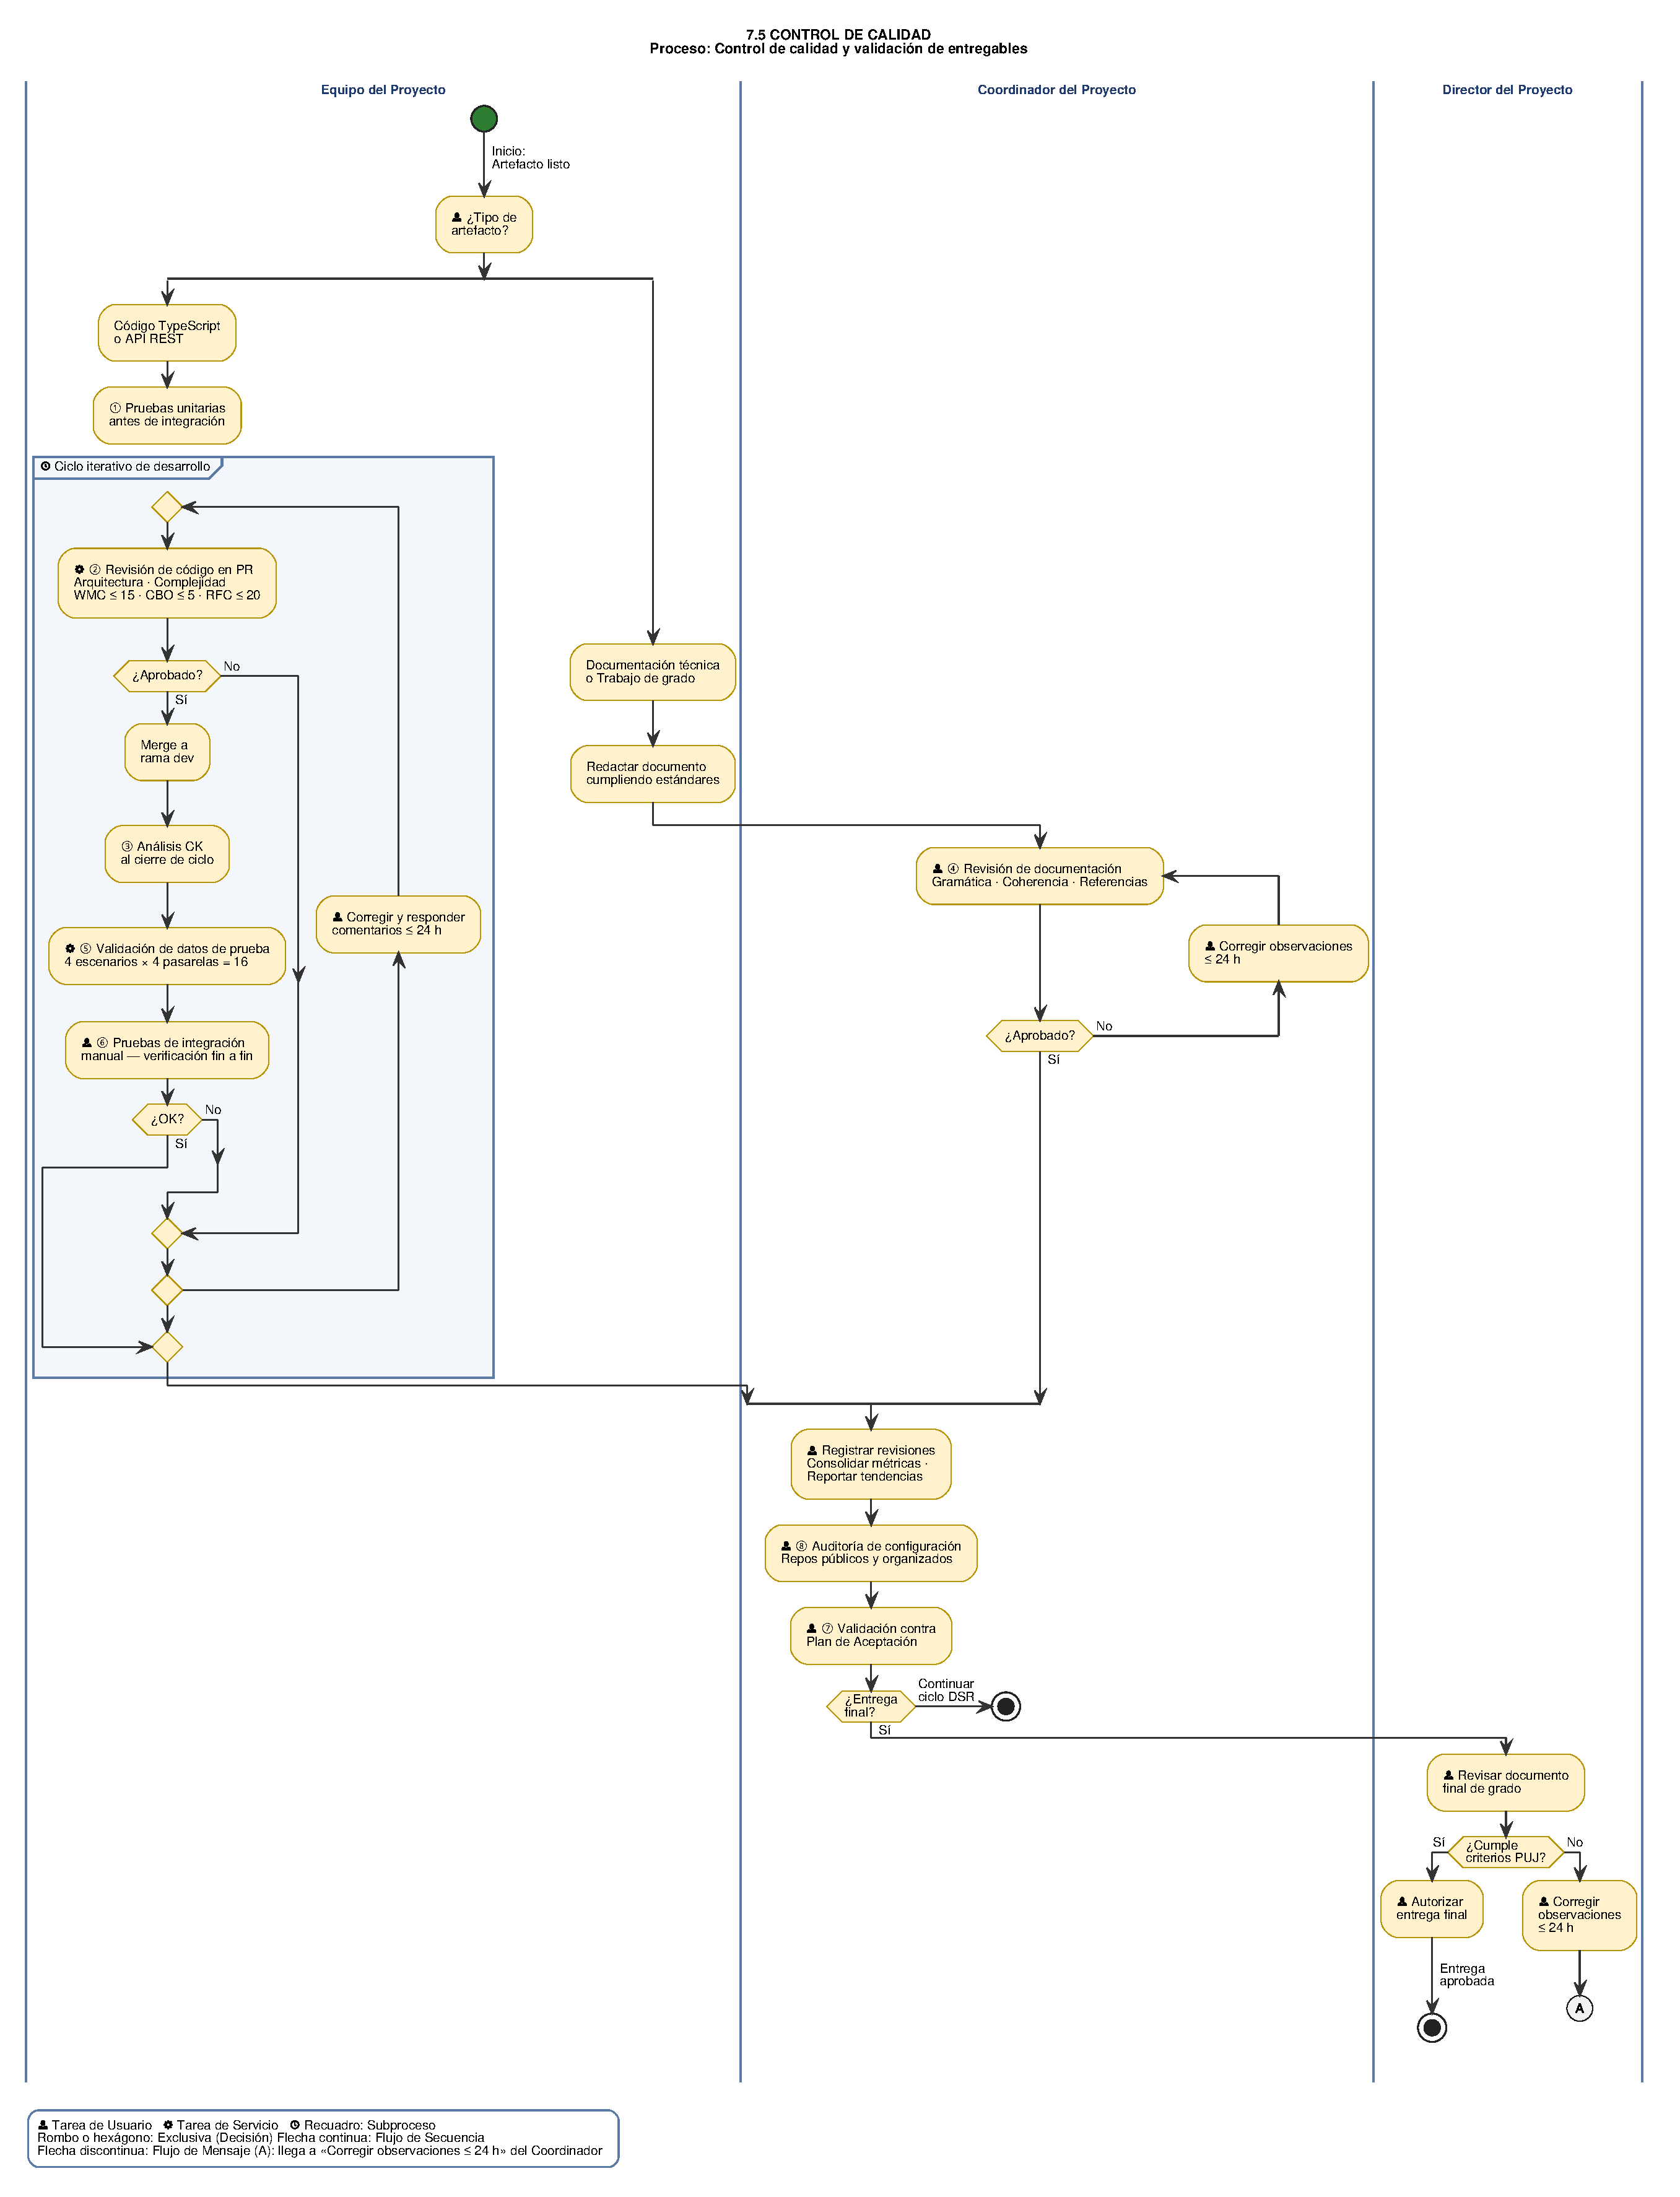
\includegraphics[width=\textwidth]{figuras/08-bpmn-calidad}
  \caption{Diagrama BPMN del proceso de control de calidad y validación de entregables}
  \label{fig:bpmn-calidad}
\end{figure}
